% Auto-generated TikZ Scatter Plot
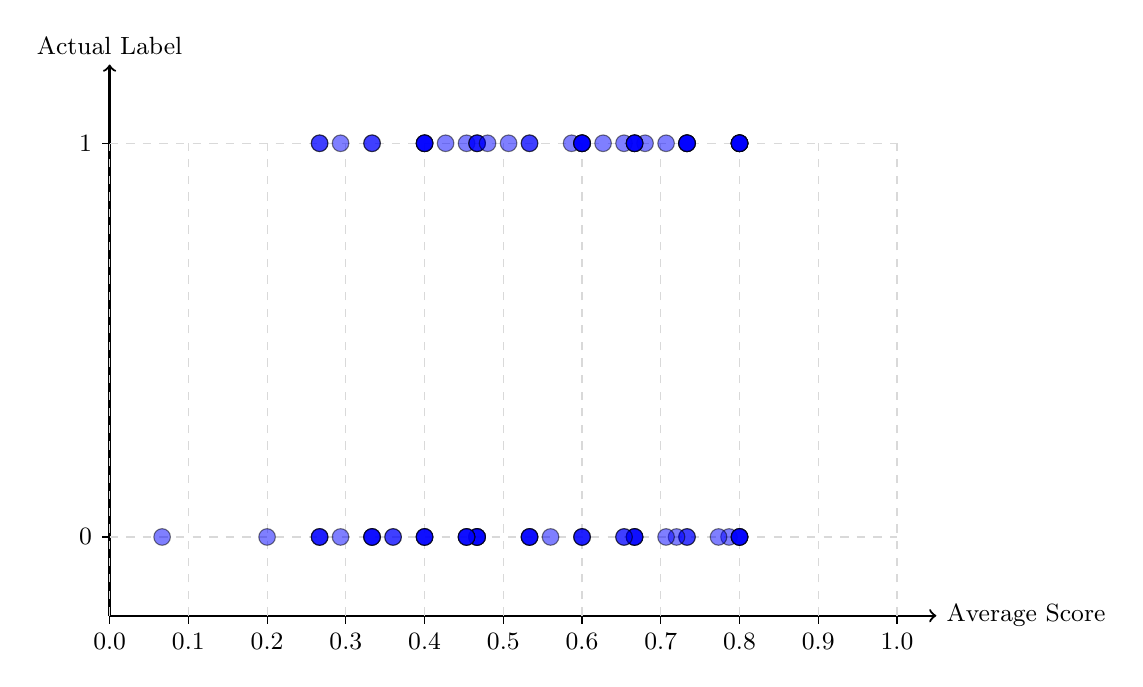
\begin{tikzpicture}
\draw[thick,->] (0,-1) -- (10.5,-1) node[right] {\small Average Score};
\draw[thick,->] (0,-1) -- (0,6) node[above] {\small Actual Label};
\draw (0, -0.9) -- (0, -1.1) node[below] {\small 0.0};
\draw[dashed, gray!30] (0, -1) -- (0, 5);
\draw (1, -0.9) -- (1, -1.1) node[below] {\small 0.1};
\draw[dashed, gray!30] (1, -1) -- (1, 5);
\draw (2, -0.9) -- (2, -1.1) node[below] {\small 0.2};
\draw[dashed, gray!30] (2, -1) -- (2, 5);
\draw (3, -0.9) -- (3, -1.1) node[below] {\small 0.3};
\draw[dashed, gray!30] (3, -1) -- (3, 5);
\draw (4, -0.9) -- (4, -1.1) node[below] {\small 0.4};
\draw[dashed, gray!30] (4, -1) -- (4, 5);
\draw (5, -0.9) -- (5, -1.1) node[below] {\small 0.5};
\draw[dashed, gray!30] (5, -1) -- (5, 5);
\draw (6, -0.9) -- (6, -1.1) node[below] {\small 0.6};
\draw[dashed, gray!30] (6, -1) -- (6, 5);
\draw (7, -0.9) -- (7, -1.1) node[below] {\small 0.7};
\draw[dashed, gray!30] (7, -1) -- (7, 5);
\draw (8, -0.9) -- (8, -1.1) node[below] {\small 0.8};
\draw[dashed, gray!30] (8, -1) -- (8, 5);
\draw (9, -0.9) -- (9, -1.1) node[below] {\small 0.9};
\draw[dashed, gray!30] (9, -1) -- (9, 5);
\draw (10, -0.9) -- (10, -1.1) node[below] {\small 1.0};
\draw[dashed, gray!30] (10, -1) -- (10, 5);
\draw (0.1, 0) -- (-0.1, 0) node[left] {\small 0};
\draw (0.1, 5) -- (-0.1, 5) node[left] {\small 1};
\draw[dashed, gray!30] (0, 0) -- (10, 0);
\draw[dashed, gray!30] (0, 5) -- (10, 5);
\fill[blue, opacity=0.5, draw=black] (6.667, 0.000) circle (3pt);
\fill[blue, opacity=0.5, draw=black] (3.333, 0.000) circle (3pt);
\fill[blue, opacity=0.5, draw=black] (4.667, 0.000) circle (3pt);
\fill[blue, opacity=0.5, draw=black] (6.000, 0.000) circle (3pt);
\fill[blue, opacity=0.5, draw=black] (3.333, 0.000) circle (3pt);
\fill[blue, opacity=0.5, draw=black] (3.600, 0.000) circle (3pt);
\fill[blue, opacity=0.5, draw=black] (4.667, 0.000) circle (3pt);
\fill[blue, opacity=0.5, draw=black] (6.667, 0.000) circle (3pt);
\fill[blue, opacity=0.5, draw=black] (7.333, 0.000) circle (3pt);
\fill[blue, opacity=0.5, draw=black] (8.000, 0.000) circle (3pt);
\fill[blue, opacity=0.5, draw=black] (4.000, 0.000) circle (3pt);
\fill[blue, opacity=0.5, draw=black] (7.333, 0.000) circle (3pt);
\fill[blue, opacity=0.5, draw=black] (4.667, 0.000) circle (3pt);
\fill[blue, opacity=0.5, draw=black] (7.867, 0.000) circle (3pt);
\fill[blue, opacity=0.5, draw=black] (4.667, 0.000) circle (3pt);
\fill[blue, opacity=0.5, draw=black] (3.600, 0.000) circle (3pt);
\fill[blue, opacity=0.5, draw=black] (2.667, 0.000) circle (3pt);
\fill[blue, opacity=0.5, draw=black] (6.000, 0.000) circle (3pt);
\fill[blue, opacity=0.5, draw=black] (4.000, 0.000) circle (3pt);
\fill[blue, opacity=0.5, draw=black] (2.667, 0.000) circle (3pt);
\fill[blue, opacity=0.5, draw=black] (8.000, 0.000) circle (3pt);
\fill[blue, opacity=0.5, draw=black] (8.000, 0.000) circle (3pt);
\fill[blue, opacity=0.5, draw=black] (7.200, 0.000) circle (3pt);
\fill[blue, opacity=0.5, draw=black] (7.733, 0.000) circle (3pt);
\fill[blue, opacity=0.5, draw=black] (4.667, 0.000) circle (3pt);
\fill[blue, opacity=0.5, draw=black] (6.000, 0.000) circle (3pt);
\fill[blue, opacity=0.5, draw=black] (6.533, 0.000) circle (3pt);
\fill[blue, opacity=0.5, draw=black] (5.333, 0.000) circle (3pt);
\fill[blue, opacity=0.5, draw=black] (2.933, 0.000) circle (3pt);
\fill[blue, opacity=0.5, draw=black] (3.333, 0.000) circle (3pt);
\fill[blue, opacity=0.5, draw=black] (6.667, 0.000) circle (3pt);
\fill[blue, opacity=0.5, draw=black] (5.600, 0.000) circle (3pt);
\fill[blue, opacity=0.5, draw=black] (4.000, 0.000) circle (3pt);
\fill[blue, opacity=0.5, draw=black] (5.333, 0.000) circle (3pt);
\fill[blue, opacity=0.5, draw=black] (4.533, 0.000) circle (3pt);
\fill[blue, opacity=0.5, draw=black] (0.667, 0.000) circle (3pt);
\fill[blue, opacity=0.5, draw=black] (8.000, 0.000) circle (3pt);
\fill[blue, opacity=0.5, draw=black] (6.667, 0.000) circle (3pt);
\fill[blue, opacity=0.5, draw=black] (5.333, 0.000) circle (3pt);
\fill[blue, opacity=0.5, draw=black] (5.333, 0.000) circle (3pt);
\fill[blue, opacity=0.5, draw=black] (4.000, 0.000) circle (3pt);
\fill[blue, opacity=0.5, draw=black] (4.533, 0.000) circle (3pt);
\fill[blue, opacity=0.5, draw=black] (3.333, 0.000) circle (3pt);
\fill[blue, opacity=0.5, draw=black] (2.000, 0.000) circle (3pt);
\fill[blue, opacity=0.5, draw=black] (4.533, 0.000) circle (3pt);
\fill[blue, opacity=0.5, draw=black] (2.667, 0.000) circle (3pt);
\fill[blue, opacity=0.5, draw=black] (4.533, 0.000) circle (3pt);
\fill[blue, opacity=0.5, draw=black] (7.067, 0.000) circle (3pt);
\fill[blue, opacity=0.5, draw=black] (6.533, 0.000) circle (3pt);
\fill[blue, opacity=0.5, draw=black] (8.000, 0.000) circle (3pt);
\fill[blue, opacity=0.5, draw=black] (8.000, 5.000) circle (3pt);
\fill[blue, opacity=0.5, draw=black] (7.067, 5.000) circle (3pt);
\fill[blue, opacity=0.5, draw=black] (6.000, 5.000) circle (3pt);
\fill[blue, opacity=0.5, draw=black] (7.333, 5.000) circle (3pt);
\fill[blue, opacity=0.5, draw=black] (6.667, 5.000) circle (3pt);
\fill[blue, opacity=0.5, draw=black] (8.000, 5.000) circle (3pt);
\fill[blue, opacity=0.5, draw=black] (5.333, 5.000) circle (3pt);
\fill[blue, opacity=0.5, draw=black] (2.667, 5.000) circle (3pt);
\fill[blue, opacity=0.5, draw=black] (6.800, 5.000) circle (3pt);
\fill[blue, opacity=0.5, draw=black] (4.533, 5.000) circle (3pt);
\fill[blue, opacity=0.5, draw=black] (5.867, 5.000) circle (3pt);
\fill[blue, opacity=0.5, draw=black] (2.667, 5.000) circle (3pt);
\fill[blue, opacity=0.5, draw=black] (4.000, 5.000) circle (3pt);
\fill[blue, opacity=0.5, draw=black] (6.533, 5.000) circle (3pt);
\fill[blue, opacity=0.5, draw=black] (4.667, 5.000) circle (3pt);
\fill[blue, opacity=0.5, draw=black] (6.000, 5.000) circle (3pt);
\fill[blue, opacity=0.5, draw=black] (7.333, 5.000) circle (3pt);
\fill[blue, opacity=0.5, draw=black] (8.000, 5.000) circle (3pt);
\fill[blue, opacity=0.5, draw=black] (7.333, 5.000) circle (3pt);
\fill[blue, opacity=0.5, draw=black] (3.333, 5.000) circle (3pt);
\fill[blue, opacity=0.5, draw=black] (4.000, 5.000) circle (3pt);
\fill[blue, opacity=0.5, draw=black] (6.000, 5.000) circle (3pt);
\fill[blue, opacity=0.5, draw=black] (6.667, 5.000) circle (3pt);
\fill[blue, opacity=0.5, draw=black] (7.333, 5.000) circle (3pt);
\fill[blue, opacity=0.5, draw=black] (6.667, 5.000) circle (3pt);
\fill[blue, opacity=0.5, draw=black] (8.000, 5.000) circle (3pt);
\fill[blue, opacity=0.5, draw=black] (4.000, 5.000) circle (3pt);
\fill[blue, opacity=0.5, draw=black] (4.667, 5.000) circle (3pt);
\fill[blue, opacity=0.5, draw=black] (4.000, 5.000) circle (3pt);
\fill[blue, opacity=0.5, draw=black] (6.000, 5.000) circle (3pt);
\fill[blue, opacity=0.5, draw=black] (7.333, 5.000) circle (3pt);
\fill[blue, opacity=0.5, draw=black] (8.000, 5.000) circle (3pt);
\fill[blue, opacity=0.5, draw=black] (4.267, 5.000) circle (3pt);
\fill[blue, opacity=0.5, draw=black] (6.667, 5.000) circle (3pt);
\fill[blue, opacity=0.5, draw=black] (8.000, 5.000) circle (3pt);
\fill[blue, opacity=0.5, draw=black] (5.067, 5.000) circle (3pt);
\fill[blue, opacity=0.5, draw=black] (8.000, 5.000) circle (3pt);
\fill[blue, opacity=0.5, draw=black] (8.000, 5.000) circle (3pt);
\fill[blue, opacity=0.5, draw=black] (4.667, 5.000) circle (3pt);
\fill[blue, opacity=0.5, draw=black] (2.933, 5.000) circle (3pt);
\fill[blue, opacity=0.5, draw=black] (4.800, 5.000) circle (3pt);
\fill[blue, opacity=0.5, draw=black] (5.333, 5.000) circle (3pt);
\fill[blue, opacity=0.5, draw=black] (6.667, 5.000) circle (3pt);
\fill[blue, opacity=0.5, draw=black] (6.000, 5.000) circle (3pt);
\fill[blue, opacity=0.5, draw=black] (3.333, 5.000) circle (3pt);
\fill[blue, opacity=0.5, draw=black] (4.000, 5.000) circle (3pt);
\fill[blue, opacity=0.5, draw=black] (6.000, 5.000) circle (3pt);
\fill[blue, opacity=0.5, draw=black] (8.000, 5.000) circle (3pt);
\fill[blue, opacity=0.5, draw=black] (7.333, 5.000) circle (3pt);
\fill[blue, opacity=0.5, draw=black] (6.267, 5.000) circle (3pt);
\end{tikzpicture}